\chapter[Conclusion]{Conclusion}\label{c:conclusion}

As this dissertation draws to a close, it is worth reflecting on the context in which this research took place. This was a period of remarkably rapid change within the field of generative AI. Undoubtedly, the most significant period of progress so far in the field, and arguably one of the most rapid technological developments in history. This rapid advancement has amplified the relevance and urgency of the findings presented in this conclusion. Similarly, it has provided valuable insights beyond the experiments carried out throughout this thesis, which are readily discussed and integrated in this conclusion and discussions. 

At the beginning of this thesis, in 2021, generative AI was expected to significantly impact many areas of our lives. At the close of it, in 2025, it is already doing so: from how we work, how we consume information, and particularly relevant for this thesis, how we create.

Against this backdrop, the question of the interface becomes ever more relevant. As I discussed throughout this thesis, how we interact with these systems largely determines their usefulness, their effectiveness and the role they play in our creative processes. 

However, so far, there are no interaction design principles focused on generative AI tools that effectively co-create with people. This has been the core research question: 

\begin{quote}
\emph{How can we design generative AI systems that act as effective co-creators, maintaining human involvement and agency while effectively leveraging the potential of this technology?}
\end{quote}

Broken down into the following subquestions: 

\begin{quote}
\textbf{Sub-Questions:}
\begin{enumerate}
    \item \emph{What is the potential of modeling dialogue in interaction design to enable effective human--AI co-creativity?}
    \item \emph{Which design principles can guide the development of co-creative systems?}
    \item \emph{What roles can humans and AI assume in co-creative processes, and in what ways can generative AI function as a co-creator?}
\end{enumerate}
\end{quote}

I examined these question through a mixed-methodology approach, developing and testing prototypes with users from a design research perspective, and engaging in creative practice through collaborations with teams working on real-world creative productions.

In the sections that follow, I will undertake two tasks. First, I will summarise and discuss the research presented thus far. Second, I will specifically address each of the three research questions.  

\section{Summary and Discussion of the Research}

In Chapter 1, I established three research questions for this thesis:

\begin{enumerate}
    \item What are the design principles that can guide the development of effective generative AI systems that are co-creative with people?
    \item What is the potential of modelling dialogue in interaction design to enable effective human–AI co-creativity?
    \item What roles can humans and AI assume in co-creative processes?
\end{enumerate}

While the primary objective of this thesis was to derive design principles for effective co-creative systems, the research was conducted as part of a broader Australian Research Council (ARC) funded project specifically focused on the potential of dialogic interaction. The central premise was to investigate how cycles of mutual influence, understanding, and communication, akin to those in human collaboration, could be enabled with generative AI systems to enhance co-creativity. Consequently, this dialogic lens was used to frame further inquiry.

\subsubsection{\textbf{Chapter 2: Literature Review}}

With the research questions and problem space defined, Chapter 2 undertook a literature review covering human creativity, computational creativity, human-computer interaction and the emerging field of human-AI co-creativity. This review revealed that while a number of design principles guide general human-computer interaction (HCI), and human-AI interaction, there are no principles specifically focused on informing the design of co-creative AI systems.

As a result, the literature review then focused on analysing emerging empirical literature to identify factors that influence the effectiveness of interaction with artificial intelligence in creative activities. 

The review also covered the literature on dialogic interaction, highlighting that dialogue has long been recognised as an effective mechanism for human collaboration and co-creativity, and numerous authors have similarly proposed its utility for modelling human-computer interaction. However, dialogic interaction remained largely undefined as an interaction design concept. 

\subsubsection{\textbf{Chapter 3: Formalising Dialogic Interaction for HCI}}

In chapter 3, I developed a formal conceptualisation of dialogic interaction in the context of co-creatiity, drawing from the theory on dialogue and empirical research in HCI 

This theoretically and empirically grounded formalisation aimed to provide a useful construct for designing systems capable of engaging in creative dialogues with users. In a subsequent section, I come back to this and discuss more specifically the answer to research question 2, discussing the potential of dialogue to enhance human-AI co-creativity that emerged from this research. 

\subsubsection{\textbf{Chapter 4: Early Experiments in Co-Creative Writing}}

While Chapters 2 and 3 focused on reviewing literature and establishing theoretical foundations, Chapter 4 transitioned to practical implementation and testing of some of these ideas through experimentation.

\textbf{Narrative Device: Combinatorial Creativity in the Wild}

The first prototype and experiment conducted was Narrative Device in early 2022. This was a simple online tool allowing users to generate a short story based on two input concepts. Shared publicly on social media, the intention was to test such a co-creative tool "in the wild." The tool went "viral": the sharing post received more than 5 million impressions, 292k engagement, 11 thousand likes, and more than 8 thousand retweets of people sharing their stories. The tool itself was used to generate over two million unique stories by more than 100,000 thousand users. This viral reception illuminated several aspects useful for human-AI co-creativity:

\begin{enumerate}
    \item \textbf{The "Wow" Factor and Bridging the Capability-Perception Gap:} This viral moment crucially occurred before the widespread public awareness of language models (ChatGPT was only released later that year). For many users, then, this was their first interaction with such a language model, which can explain its reception. As I discussed in Chapter 2 and 3, a gap often exists between a model's actual capabilities and perceived capabilities: interfaces are often responsible for bridging this gap. Narrative Device's success was partly attributable to this, as many users were unaware that language models creative capabilities.
    \item \textbf{Simplicity and Clarity of Interface:} The interface was intentionally simple: two text boxes and a generation button. This made the system's capabilities clear, addressing the capability-limitations gap and providing distinct visibility about what the system could do well. This contrasts with more recent open-ended prompt boxes that can provide the illusion that the system can simply do anything, leading to frustration arising from unmet expectations. Moreover, a primary intention was for the tool to be fun, a crucial element for effective creativity as discussed in Chapter 2. The interface design was unintimidating and encouraged playfulness. 
    \item \textbf{Enabling Combinatorial Creativity:} The interface design, requiring users to provide two concepts for the AI to combine, proved to be an effective way to leverage both human and computational creativity. This aligns with Margaret Boden's concept of combinatorial creativity and the general understanding of creativity as the novel combination of existing elements.
    \item \textbf{The audience sharing effect}: the virality of the tool was partly explained by the fact that the output story, along with the inputs, could be screenshoted and easily shared in social media. People then were, in a sense, proud to share the concepts they had come up with and how the tool had integrated them into a story. This was unintentional. But it highlighted that usage of a co-creative tool largely depends on the willingness of people to share it's outputs, and share their process using the tool. Computational creativity researchers have proposed that framing and impact are important vectors to consider when designing these systems.\cite{Colton2011-uy, Jordanous2016-xb} This experiment showed this in practice. Indeed, co-creativity never happens in a vacuum, and it is influenced by the cultural enviroment. 
\end{enumerate}
\textbf{Beyond Chat: Shared Creative Workspaces for Writing}

Following the Narrative Device experiment, and particularly after the release of ChatGPT in late 2022 which led to the widespread adoption of LLMs and the convergence towards chat-based interaction as the dominant paradigm, I developed a second co-writing experiment. As a hypothesis, I observed that while chat interfaces facilitated communication, they might be limited for co-creative writing because they lacked a dedicated space for the co-creation itself, beyond the linear message stream. This often relegated users to the role of an "outsourcer," providing instructions rather than directly engaging in the writing, simply because a shared space for contribution was absent.

To investigate this, I prototyped a tool featuring both a chat window for communication \textit{about} the artefact and a shared text editor for co-creation \textit{through} the artefact. In a comparative user study against a chat-only prototype, several findings emerged:

\begin{enumerate}
    \item \textbf{Shared collaborative spaces in addition to chat can lead to more user involvement:} The study indicated that providing distinct spaces for communication and direct contribution led to increased user involvement. Users of the shared editor prototype were more likely to report that the final written piece contained their own words, whereas chat-only users often felt the AI had done most of the work. This supported the idea of a shared creative space, echoing concepts from the theory of dialogue discussed in Chapter 3.
    \item \textbf{The Challenge of User Involvement and Cognitive Offloading:} Despite the hybrid interface leading to more user involvement, a tendency for users to report that the AI did most of the work persisted. This aligns with a broader trend identified in emerging literature, where users opt for paths of least resistance, leading to cognitive offloading and over-reliance, leading to skill degradation and reduced enjoyment. While interface design can mitigate this, it may not eliminate it entirely, highlighting a fundamental tension in AI-assisted creativity.
    \item \textbf{Managing AI Contributions:} The shared editor interface, while fostering involvement, introduced the challenge of AI making destructive contributions. Users expressed a desire for mechanisms to review, accept, or reject AI edits, akin to version control in collaborative software. This insight was later echoed by the development of tools like Cursor for co-programming, which implemented such features.
    \item \textbf{Beyond Textual Prompts:} Participants noted the potential benefits of GUI elements to trigger specific AI actions (e.g., rephrasing, editing), not only for convenience but for clearer visibility of what the AI can actually do. 
\end{enumerate}

\subsubsection{\textbf{Chapter 5: Co-Creativity in Visual Domains}}

In Chapter 5, the research focus shifted to visual creativity and image generation, explored through two professional case studies.

\textbf{The Australian Financial Review: "Impossible Photography"}

This collaboration involved producing AI-generated "impossible photography" portraits for the AFR Magazine's 2023 Power List issue, including the cover of the paper and the magazine. The aims were twofold: to explore novel creative possibilities afforded by AI (e.g., metaphorical portraits unachievable with traditional photography, such as the Reserve Bank Governor piloting a hot air balloon symbolising inflation control) and to stimulate discussion about the ethical implications of deepfakes. Crucially, the magazine still employed photographers to produce the portraits that are now a staple of the annual issue. 

This real-world professional use case yielded several critical insights:

\begin{enumerate}
    \item \textbf{Control and Multimodality:} Achieving desired stylistic and compositional control with text-only prompts proved challenging. After trying multiple tools, the workflow ultimately relied on tools that allowed image-to-image generation, using reference images to guide subject position and style, underscoring the limitations of purely textual control and the need for multimodal input.
    \item \textbf{Iteration and Refinement:} Generative models, particularly at the time, were not optimised for iterative editing but rather for generating new outputs. Refining specific aspects of an image while preserving others was a significant hurdle, often necessitating manual post-processing in Photoshop.
    \item \textbf{Consistency:} Ensuring consistent subject likeness, especially when the individuals were not heavily represented in the AI's training data, was a major challenge. It required training bespoke models for each subject, with considerable effort to achieve acceptable resemblance, while highlighting the increasing accessibility of training models to produce deepfakes undistinguishable from real photographs. 
    \item \textbf{Public Perception:} The publication of these images sparked considerable public discussion. While the deepfake aspect was a concern, a more vocal segment of the negative reaction centred on the perceived replacement of human photographers. This highlighted the influence of public perception (Rhodes' "Press") on the adoption and impact of creative AI and how the framing of work involving AI is crucial (a point similarly addressed in the Narrative Device experiment). The magazine itself provided an entire section explaining the process, and the intention of the work, but this framing was lost in social media dissemination, leading to more negative reactions. This suggests designers must consider not only the system but also how its outputs are framed and perceived, potentially by designing systems that are ethically trained and encourage attribution and transparency about the human involvement.
\end{enumerate}

\textbf{Tilly: An AI Co-Creator for Interior Design}

The second case study in this chapter involved a collaboration with a Sydney-based interior design studio to develop "Tilly," an AI co-creator. Tilly, an LLM-powered chatbot, assisted the studio in ideating conceptual and visual solutions for design briefs, with the specific intention to produce designs for exhibition at Milan Design Week. This case study yielded similar insights about the value of framing outputs, and the challenges of controlling and iterating on outputs. 

Designers at Studio Snoop used Tilly to ideate and ultimately produce a set of five designs, printed and exhibited at a venue within the design week. In front of each design and around the venue, iPads were placed were visitors could chat with Tilly, who was able to explain and frame the designs. Tilly was also able to ask for and collect feedback from participants. This feedback was synthesised by Tilly and relayed to the designers in Sydney, who iterated on the designs daily. This process resulted in five final designs produced through an interaction between the designers, the AI, the audience, and myself as the system designer. Importantly, these designs were then physically produced by different artisans and studios around the world. and exhibited at London Design Festival, bringing in new actors in a collective network of co-creativity partly enabled by generative language models. 

Learnings from this case study included:

\begin{enumerate}
    \item \textbf{Novel AI Roles for AI, involving the audience and framing outputs:} AI demonstrated novel potential to take on a roles humans cannot easily fulfill, such as framing the outputs for an audience in parallel, and collecting, synthesising and interpreting large amounts of feedback data from an audience. This again can be understood as bringing Rhode's Press more explicitly into the creative interaction, enabling a novel form of distributed, collective, iterative co-creativity.
    \item \textbf{The value of ideation and the challenge of iteraton and control}: Tilly provded useful as a visual ideation partner, helping designers explore multiple possibilities rapidly to fulfil the brief. However, designers found it was notably difficult to hone in specific promising directions, by iterating on outputs while maintaining other elements consistent. Such iterative honing on creative avenues is crucial in creative processes, and as the AFR case study also showed, remain a crucial limitation of generative AI in co-creativity. 
\end{enumerate}

\subsubsection{\textbf{Chapter 6: New Media Installations – AI in Context-Aware Sonic Art}}

Chapter 6 detailed my practice-based research into new media installations, exploring the idea of AI interacting with and responding to wider environmental systems. These installations used LLMs to ingest complex data from the surrounding environment and interpret it to drive the generation of continuous soundscapes.

\begin{enumerate}
    \item \textbf{System of a Sound (Canberra):} This installation ingested real-time data related to local weather, CO2 levels, national economic indicators, and social media activity. The soundscape reacted to these inputs, with different data streams affecting various layers of the soundscape at different paces, inspired by Stewart Brand's theory of Pace Layers. An interactive component allowed the audience to influence the soundscape through body pose and gestures.
    \item \textbf{Music of the Sails (Sydney Opera House):} This installation focused on data from the Opera House building itself (energy use, water consumption, performance schedules) to generate a continuous, evolving soundscape.
\end{enumerate}

Importantly, the music generated by the system was produced or curated by human composers, and included in a music engine that the AI could then influence based on the interpretations of data. 

The intention of these installations was not to simply create an "AI-generated installation". Instead, we used the language models as a tool and co-creator, enabling a new type of creative operation: that of semantically interpreting complex data to drive a sonificiation process. Importantly, it yielded a number of limitations for this type of practice, primarily around steering and control: given the outputs were distributed across relatively long periods of time, it was difficult to understand and steer them. For example, only after a few days it became clear that the model was fixating on a specific undesirable output. Steering it away fro that behavior proved challenging. This sort of behavior is both a "feature and a bug" of these systems. Weisz terms this "generative variabilty" \cite{Weisz2024-io}, and the unpredictability of these systems is at least for now, the price to pay for richer semantic possibilities in sonficiation and creative production in general using these tools. 


\section{Research Question 1: Design Principles for Co-Creative AI Systems}


Design principles serve as crucial research outputs that bridge the gap between theory and practical application. The intention underpinning the principles formulated in this thesis is that they will be embraced by the wider community of interaction designers, engineers, researchers, entrepreneurs, and indeed, anyone considering the implementation of artificial intelligence in scenarios where co-creativity with humans is desired. This implies a context where the aim is to maintain and enhance human creativity and involvement, synergising these with the unique creative capacities of machines, rather than seeking to replace human creative agency.

This objective is particularly relevant in light of the emerging trends discussed in Chapter 2, where an increasing proclivity for over-reliance on AI models has been observed, potentially leading to skill degradation, diminished user involvement, and ultimately, undesirable creative outcomes. As demonstrated in Chapter 4, this lack of user involvement can be, at least in part, attributed to prevailing interaction designs.

The principles enumerated below are not intended as an exhaustive or immutable list. They do intend to fill the gap in principles for effective co-creative AI systems, but it is my hope that they will not be taken as fixed, and instead stimulate further discussion, challenges and expansion. Ultimately, I believe this discussion addresses what is arguably one of the most important questions of our time: how to augment, rather than supplant, human creativity in the context of highly capable artificial intelligence.


% Add these to your document preamble:
% Add these to your document preamble:

\renewcommand{\arraystretch}{1.4} % increase row height

\begin{table}[ht]
  \centering
  \rowcolors{2}{gray!15}{white} % alternating row colors
  \begin{tabularx}{0.95\textwidth}{>{\centering\arraybackslash}p{0.25\textwidth} X}
    \rowcolor{blue!20}
    \textbf{Principle} & \textbf{Description} \\ \midrule
    Visibility & Provide Clear Visibility of AI Capabilities and Limitations \\
    Style & Allow Users to Define and Maintain Their Stylistic Voice \\
    Expression & Provide Expressive, Playful, and Multimodal Interfaces \\
    Iteration & Support Guided Exploration and Iteration \\
    Involvement & Encourage User Effort and Involvement \\
    New Possibilities & Prioritise New Creative Possibilities Over Automation of Existing Tasks \\
    Shared Spaces & Provide Shared Collaborative Spaces for Interaction \emph{Through} and \emph{About} the Creation \\
    Changes & Manage AI Contributions Effectively, Non-Destructively, and Track Changes \\
    Workspace Integration & Integrate Within Users’ Workspaces and Workflows \\
    Context Awareness & Integrate into the User’s Wider Context \\
    Perception & Consider Creator and Audience Perception; Frame Outputs and Human Involvement \\
    Ethics & Consider the Ethical Dimension and Impact on the Creative Ecosystem \\ \bottomrule
  \end{tabularx}
  \caption{Core design principles for human–AI co-creative interfaces}
  \label{tab:co_creative_principles}
\end{table}





\begin{enumerate}[label=\arabic*., wide, labelindent=0pt]

\item \textbf{Visibility: Provide Clear Visibility of AI Capabilities and Limitations:}
    \begin{itemize}[label=\textbullet, leftmargin=*]
        \item \textbf{Principle:} Interfaces should clearly and simply communicate what an AI system can and cannot do, how users can interact with it, and the likely outcomes of their actions. This helps align user expectations with actual AI capabilities, fostering more effective interaction.
        \item \textbf{Rationale \& Examples:} The initial success of the Narrative Device prototype (Chapter 4) can be partly attributed to its interface, which clearly demonstrated its contrained capability. This helped bridge the common gap between what users perceive an AI can do and its actual functionalities. Participants in subsequent co-writing experiments (Chapter 4) also expressed a desire for clearer affordances, such as GUI elements that trigger specific AI actions, rather than relying solely on open-ended prompts which can imply limitless capability. If generative systems are complex systems with vast latent potential, the role of the interaction and interface designers is not only to provide a "door" to the them, but also a "map" to navigate its potential. Effectively designed interfaces are essential for users to gracefully navigate the "jagged technological frontier" that AI presents, ensuring that the performance and effectiveness of the interaction hinge on an informed understanding of the model's strengths and boundaries \cite{DellAcqua2023-og}. Beyond this research extensive literature highlights how a better understanding of capabilities and limitations of generatve systems leads to more involvement and better outcomes. In Amershi's Guidelines for Human-AI interaction stated, as it's first two principles: making clear what the system can do, and how well it can it \cite{Amershi2019-wu}. Similarly, and not surprisingly, these observations align with the well established principle of visibility in user interface design \cite{Nielsen1994-df}. For similar and also distinct reasons, this principle remains crucially important for co-creativity. 
    \end{itemize}

\item \textbf{Style: Allow Users to Define and Maintain Their Style}
    \begin{itemize}[label=\textbullet, leftmargin=*]
        \item \textbf{Principle:} Co-creative systems should empower users to define, refine, and maintain their personal or brand-specific creative style throughout the creative process, ensuring outputs align with their unique aesthetic, voice and preferences.
        \item \textbf{Rationale \& Examples:} A frequently observed challenge across studies was the difficulty users faced in stylistically steering model outputs to reflect their own voice. In the co-writing experiments (Chapter 4), participants often reported that AI-generated text did not sound "like their own writing," which diminished their sense of agency, contribution, and ownership. Similarly, in the AFR case study (Chapter 5), significant effort was dedicated to aligning AI-generated visuals with the magazine's established stylistic guidelines. The sonic installations (Chapter 6) also prioritizsed maintaining a distinct compositional identity; human collaborators carefully composed and curated the sound palette available to the generative music engine, ensuring the AI's combinatorial explorations remained within a defined artistic style. Successful co-creation hinges on enabling users to produce work aligned with their personal style, fostering a sense of craft and ownership over the final artefact.
    \end{itemize}

\item \textbf{Expression: Provide Expressive, Playful, and Multimodal Interfaces}
    \begin{itemize}[label=\textbullet, leftmargin=*]
        \item \textbf{Principle:} Design interfaces that move beyond text-only interaction, offering users expressive, playful, and multimodal ways to engage with generative AI, control outputs, and explore new creative possibilities.
        \item \textbf{Rationale \& Examples:} The current paradigm of text-based interaction with generative AI is often limited, particularly for creative tasks where visual or other sensory modalities are central. Designers, for instance, often identify as "visual thinkers" rather than "verbal thinkers" \cite{Park2024-gw}. In the Tilly case study, the designer's process involves curating moodboards, which then they struggled to translate into text-to-image prompts. The AFR study (Chapter 5) similarly found that achieving stylistic control and desired outputs often necessitated tools that allowed for visual references, and that text was a limited interface for this. Beyond mere control, playful and multimodal interfaces can enhance the user experience and open new avenues for creativity. The Narrative Device (Chapter 4) offered a playful interface for combining concepts, while the "System of a Sound" installation (Chapter 6) incorporated a gestural interface for audience interaction. Research also suggests that expressive navigation interfaces can better support ideation than standard text-to-image systems, even with less capable underlying models. Furthermore, generative systems excel at enabling novel forms of creative expression by translating between modes—such as data to music in the installations (Chapter 6), or emerging tools that facilitate operations like image to music modalities. Enabling users to steer outputs through multimodal control can lead to more controllable, engaging, and creatively expressive co-creative experiences.
    \end{itemize}

\item \textbf{Iteration and Exploration: Support Guided Exploration and Iteration}
    \begin{itemize}[label=\textbullet, leftmargin=*]
        \item \textbf{Principle:} Co-creative systems should facilitate iterative design processes, enabling users to explore diverse creative avenues, refine outputs, and pursue promising directions while maintaining consistency and control.
        \item \textbf{Rationale \& Examples:} Creative processes are inherently iterative, demanding exploration and refinement, especially during early ideation. However, many current AI tools hinder this, often generating isolated outputs without supporting meaningful iteration. In the co-writing experiment (Chapter 4), participants desired options to view and select from multiple AI-generated alternatives. Similarly, designers in the "Tilly" case study (Chapter 5) struggled to iterate on design variations while preserving core elements, as the AI generated entirely new images rather than allowing consistent editing. The new media installations (Chapter 6) also highlighted the need for iterative collaboration, as the language model sometimes fixated on certain outputs, requiring difficult manual intervention to steer it while retaining desired characteristics. While some limitations are technical (e.g., AI models struggling with non-destructive edits), design can contribute to mitigating these. This includes enabling outputs to serve as inputs for further refinement, providing "tree-like" generation structures for exploring branching possibilities, or maintaining rich histories of interaction to revert to or branch from different states. This approach fosters essential feedback loops, moving beyond linear, isolated generations towards a more dynamic and responsive co-creative dialogue.
    \end{itemize}

\item \textbf{Encourage User Effort and Involvement:}
    \begin{itemize}[label=\textbullet, leftmargin=*]
        \item \textbf{Principle:} Design co-creative systems to actively encourage and reward user effort and involvement, mitigating the risks of cognitive offloading and fostering deeper engagement and skill development.
        \item \textbf{Rationale \& Examples:} A significant pitfall of interacting with generative AI systems is the potential for cognitive offloading, leading to reduced user effort and engagement. Tools that can effectively incentivize and leverage user effort are therefore invaluable. The Narrative Device (Chapter 4) was designed with this intent: while capable of autonomous story generation, its core interaction encouraged users to engage in divergent thinking by combining disparate concepts—a cognitively demanding and creative act. The tool then rewarded this effort by weaving those concepts into interesting narratives. Similarly, in the co-writing experiment (Chapter 4), the interface explicitly provided ample space and affordances to encourage substantial user contribution. The new media installations (Chapter 6) also emphasised human involvement by using a generative engine built upon human-composed and curated music rather than entirely synthetic sound. This focus on maintaining human contribution is crucial, as a growing body of research indicates that a lack of user involvement can lead to skill degradation and diminished performance when working with these systems. By structuring interactions to demand meaningful user input, co-creative tools can counteract these disadvantages, fostering sustained engagement and the development of symbiotic virtuosity.
    \end{itemize}

\item \textbf{Prioritise New Creative Possibilities Over Automation of Existing Tasks:}
    \begin{itemize}[label=\textbullet, leftmargin=*]
        \item \textbf{Principle:} Focus on how generative AI can enable entirely new creative possibilities, practices, and forms of expression, rather than solely automating or accelerating tasks humans already perform. Encourage the exploration of AI's unique capabilities to expand the creative palette and introduce novel creative operations.
        \item \textbf{Rationale \& Examples:} Some of the most interesting potential of co-creative AI lies not in merely automating or accelerating tasks humans already perform, but in its capacity to enable entirely new creative possibilities, creative practice, allowing creators to do new things. Designers of co-creative systems should therefore be encouraged to explore how generative AI can introduce novel creative practices and operations. The new media installations (Chapter 6) exemplified this by using AI for real-time, continuous semantic interpretation of complex data into evolving sonic art—a practice not easily achievable by humans alone—which explicitly brought the environment into the creative process. In the "Tilly" case (Chapter 5), AI facilitated a new form of iterative, collective creative practice by enabling designers to incorporate audience feedback, analyse it, and helping them frame their creations to a wider audience. Similarly, the AFR project (Chapter 5) allowed for the exploration of "impossible photography," a new type of visual practice to tell stories about subjects in ways previously difficult or impossible with a traditional camera. Narrative Device (Chapter 4) also functioned as a new instrument for narrative creativity, offering users, among other things, inspiration for their own creative writing through a tool not previously available. As discussed in the introduction, new technologies often evoke fears of automation, akin to the camera's initial reception in the world of painting, but their creative value is often realised when they enable new forms of expression and expand the palette of creative possibilities by providing new creative primitives. It is difficult to know in advance what these new possibilities may be. But interaction designers can be proactive by asking: what new things can these technologies do, that existing tools do not afford?
    \end{itemize}

\item \textbf{Provide Shared Collaborative Spaces for Interaction \textit{Through} and \textit{About} the Creation:}
    \begin{itemize}[label=\textbullet, leftmargin=*]
        \item \textbf{Principle:} Offer dedicated, interactive spaces where human and AI can directly and concurrently work \textit{on} or \textit{through} the creative artifact, distinct from channels primarily used for communication \textit{about} the artifact.
        \item \textbf{Rationale \& Examples:} Human co-creation typically involves both communication \textit{about} the work (e.g., verbal exchanges to define goals, clarify, give feedback) and direct co-creative acts \textit{through} the work itself (e.g., playing notes, writing words, drawing lines). This distinction holds value for designing human-AI co-creative systems. Historically, interaction with AI evolved from simple autocomplete or program execution. More recently, text-to-X generation and conversational interfaces (like ChatGPT) became ubiquitous. The rapid adoption of such conversational tools demonstrated the utility of bidirectional communication for interaction \textit{about} the creation, enabling users and AI to align on goals, intentions, and meanings, provide feedback, and engage with the necessary nuance for co-creation. Research, such as by Rezwana and Maher, has also shown that bidirectional communication can increase the perceived effectiveness of co-creation and feelings of collaboration. However, as argued in Chapter 4, prevailing chat interfaces often confine interaction primarily to being \textit{about} the creation, limiting direct human contribution at the artifact level, largely because a dedicated space for such contribution is lacking. The writing experiment in Chapter 4 demonstrated that providing a distinct space for co-creation increased user involvement. Such separation facilitates mixed-initiative interaction, a conceptualisation beneficial for creativity, and allows users to more readily incorporate their own voice and style, thereby maintaining their skills and engagement at the artifact level.
    \end{itemize}

\item \textbf{Manage AI Contributions Effectively, Non-Destructively, and Track Changes:}
    \begin{itemize}[label=\textbullet, leftmargin=*]
        \item \textbf{Principle:} Implement mechanisms that allow users to clearly distinguish, review, accept, reject, or version AI-generated contributions, preserving user agency and preventing the AI from destructively overwriting human work.
        \item \textbf{Rationale \& Examples:} While a shared co-creative space is beneficial, users need control over how AI contributions are integrated. In the co-writing experiment (Chapter 4), a common frustration was the AI overwriting user text. Participants expressed a need to distinguish between AI and human contributions and to manage changes, similar to features in collaborative software. Although co-creativity often implies a blending of agencies where output is not solely attributable to one actor, pragmatic collaboration requires tools that empower users. This includes the ability to accept or reject changes, revert to previous states, and iteratively steer the model. Buschek et al. (2021) identified this as a potential pitfall, terming it "conflicts of territory," such as when AI overwrites manually created or edited content. They recommend tracking user edits to protect them and confirming with the user before introducing changes, or integrating this information into the AI's inference process. Tools like Cursor, a coding IDE for AI collaboration, are a good example of successfully implementing this by showing "code diffs" and asking for user confirmation before applying AI changes, also allowing users to create checkpoints and revert if needed. This ability to undo and recover from errors aligns with established usability heuristics, such as Nielsen's, and Resnick's design principles for creative tools, which advocate for keeping rich histories of interaction and recovering from errors.
    \end{itemize}


\item \textbf{Integrate Within Users' Workspaces and Workflows:}
    \begin{itemize}[label=\textbullet, leftmargin=*]
        \item \textbf{Principle:} Co-creative tools should seamlessly integrate into users' existing professional workspaces and workflows, facilitating the orchestration of multiple tools and enhancing rather than disrupting established creative practices.
        \item \textbf{Rationale \& Examples:} Effective co-creative tools must acknowledge that creative work rarely occurs in isolation. As discussed in the literature review, orchestrating diverse tools is an emerging role for humans working with generative AI \cite{Palani2024-on}. The AFR case study (Chapter 5) exemplified this, demonstrating the necessity of connecting generative and non-generative tools within a cohesive workflow to achieve desired outcomes. Users frequently employ multiple generative AI tools in conjunction with other traditional software, forming complex pipelines. Enabling this interoperability empowers users, making their creative workflows more efficient and expanding creative possibilities. The new media installations (Chapter 6) also involved connecting various components: data acquisition and processing nodes, a Large Language Model (LLM), a human-designed music engine and visual displays. Beyond workflows of tools, integrating tools directly into familiar workspace environments, such as embedding AI features within existing Integrated Development Environments (IDEs) like Cursor, or connecting to Digital Audio Workstations (DAWs) and graphic design software, is crucial. This integration minimises friction, supports user agency, and fosters the adoption of AI tools within professional contexts.
    \end{itemize}

\item \textbf{Integrate into the User's Wider Context:}
    \begin{itemize}[label=\textbullet, leftmargin=*]
        \item \textbf{Principle:} Design co-creative systems to be aware of and responsive to their broader socio-cultural, environmental, and informational contexts, moving beyond isolated operation to become embedded, socio-technical actors in the creative process.
        \item \textbf{Rationale \& Examples:} Co-creation is influenced by the environment, cultural trends, and audience reception, which collectively shape the value and meaning of creative output. Co-creative systems should not exist in isolation but rather be designed with an awareness of their placement within this context. This underpinned the new media installations (Chapter 6): to explore how an LLM, situated within its environment, both immediate and larger, could react to and generate art directly responsive to that context. Similarly, in the "Tilly" co-creation case (Chapter 5), providing it with context about seasonal design trends and the environmental impact of different materials was crucial for the ideation of designs. For writers in the co-writing experiment (Chapter 4), a common desire was for the AI to possess greater "world awareness" and access to real-time information to produce more contextually relevant text, a limitation of the prototype's disconnected language model. Co-creative systems that can interact with and draw from their external environment become more valuable socio-technical actors, producing creative artefacts that are not only novel but also resonant with their intended context.
    \end{itemize}

\item \textbf{Consider Creator and Audience Perception; Frame Outputs and Human Involvement:}
    \begin{itemize}[label=\textbullet, leftmargin=*]
        \item \textbf{Principle:} Acknowledge and proactively address audience and creator perceptions of AI-generated content by designing mechanisms that frame the creative process, highlight human involvement, and communicate the ethical dimensions of the output.
        \item \textbf{Rationale \& Examples:} The reception of AI-generated artefacts, as seen in the AFR case study (Chapter 5) where negative associations with AI (e.g., job displacement, "stolen" work) led to backlash, significantly impacts adoption and valuation. Designers of co-creative tools must be acutely aware of how their tools are perceived and positioned within the creative ecosystem. A key strategy is to enable transparent framing of the creative process and the degree of human involvement. This includes communicating the human effort invested, the collaborative nature of the creation, and the ethical considerations underpinning the AI's development and use. Much negative sentiment towards AI stems from the perception of minimal human effort or complete automation. Therefore, co-creative tools should explicitly emphasise human agency and skill development, fostering what some research terms "symbiotic virtuosity", where users cultivate expertise in using the system akin to a traditional instrument. By foregrounding human contribution and effort, the outputs produced with these tools can be perceived and valued differently, shifting the narrative from displacement to empowered collaboration.
    \end{itemize}

\item \textbf{Consider the Ethical Dimension and Impact on the Creative Ecosystem:}
    \begin{itemize}[label=\textbullet, leftmargin=*]
        \item \textbf{Principle:} Design co-creative tools with a proactive and holistic consideration of their ethical implications and their broader impact on the creative ecosystem, fostering transparency, fair compensation, and responsible innovation.
        \item \textbf{Rationale \& Examples:} It is increasingly imperative for designers of co-creative tools to address the ethical dimensions of their creations. This encompasses designing tools that are ethically trained, transparent about their data sources, and provide fair compensation to artists whose work contributes to training datasets. Such considerations are vital for fostering trust and acceptance among creators and audiences alike. Across multiple case studies in this research, ethical concerns were a recurring theme. In the Narrative Device experiment (Chapter 4), questions arose regarding data provenance. The AFR project (Chapter 5) faced public criticism regarding the ethics of AI use on social media. Participants in the co-writing experiment (Chapter 4) frequently voiced concerns about copyright and the potential impact of AI on creative industries. Designers must critically assess the long-term impact of their tools on the creative ecosystem and engage with the ethical dimension in which co-creative systems are embedded.
    \end{itemize}

\end{enumerate}

\section{Research Question 2: The Potential of Dialogic Interaction for Human-AI Co-Creative Systems}

The second research question of this thesis investigated the potential of dialogic interaction to enhance human-AI co-creative systems. This research was conducted as part of an Australian Research Council (ARC) Discovery Project specifically focused on exploring the potential of dialogue in human-AI collaboration.

It is worth reflecting briefly again on the technological backdrop against which this research unfolded. Today, the concept of dialogic interaction with AI might appear self-evident; conversational interfaces are the prevalent mode of interaction with large language models, which are themselves often presented as "dialogue models." However, at the onset of this thesis, this was not the prevailing paradigm. An early experiments, detailed in Chapter 3, involved an attempt to repurpose existing autocomplete models, such as GPT-2, into dialogic co-creative authors that could in engage in a conversation. A key interest was whether these models could fluidly switch between discussing creative goals with a user and directly performing creative writing tasks within a single conversational thread. These initial explorations demonstrated a nascent capacity within generative language models for such engagement.

Yet, it also became clear that effective creative dialogue, drawing from established theories across various fields, encompasses more than simple conversational turn-taking. It necessitates mechanisms for clarification, feedback, goal alignment, and, crucially, mutual influence, as well as being able to collaborate with the user at the artefact level. Consequently, Chapter 3 also presented a deeper analysis of dialogue, synthesising literature from diverse disciplines to identify six core elements defining a rich dialogic interaction: bidirectional communication, shared collaborative spaces, mutual influence, mutual understanding, iteration, and context-awareness. This framework, rooted in HCI empirical literature and theories of dialogue, provided a conceptual lens used throughout the thesis.

The Narrative Device experiment (Chapter 4), for instance, while successful in generating public interest and demonstrating a form of combinatorial creativity, fell short of affording a truly dialogic interaction. Its one-off, non-iterable outputs limited its role, constraining it primarily to idea generation or entertainment rather than sustained co-creation. The subsequent rise of conversational interfaces like ChatGPT validated a core aspect of the dialogic hypothesis: that iterative, bidirectional communication is indeed valuable for many creative tasks. Users readily adopted these tools for a myriad of creative scenarios.

However, this widespread adoption also surfaced new challenges, as explored in the "Beyond Chat" study (Chapter 4). It became evident that a successful co-creative dialogue often requires not only a space for communication (about the creation) but also a distinct space for direct co-creation (through the artefact itself), where the creative work can be jointly manipulated and evolved. This led to a more robust understanding of dialogic interaction's value, further refined in collaborative work that distinguished between different levels of dialogue, with the most complete form involving interaction in both the language (abstract) space and the artefact (execution) space.

This framing proved useful when extending the inquiry to visual domains. Experiments and case studies (Chapter 5) revealed that early image generation systems significantly lagged behind language models in their dialogic capabilities. Most tools offered one-off generations with minimal capacity for iterative feedback or nuanced communication regarding goals and intentions. These systems were largely constrained to text-to-image or basic image-to-image interactions. This limitation is partly attributable to underlying architectures; diffusion-based models, which generate outputs from noise conditioned by prompts, differ fundamentally from the sequential transformer architectures of LLMs that more readily maintain conversational context and operate within a unified language space for both communication and artefact creation. Even in the "Tilly" case study (Chapter 5), where a chatbot was designed as a co-creator for visual design workflows, Tilly operated entirely within the language domain, assisting with prompt generation, feedback synthesis, and framing creations (all tasks at the conceptual, abstract language space), but not directly manipulating visual outputs.

As of the writing of this thesis in 2025, significant advancements are addressing these limitations. The emergence of multimodal models that operate natively across image and language spaces, sharing common token representations, is beginning to enable more fluid editing, refinement, and iterative cycles in visual generation. These systems can more seamlessly switch between language for communication and alignment, and the image space for direct creation. The same trend is unfolding in other domains, such as music. Furthermore, the rise of agentic AI, capable of controlling other creative software tools, suggests that even language-centric AIs may increasingly act within the artefact space by manipulating the tools that produce visual or other non-linguistic outputs. Indeed this was the approach I took for the installations discussed in Chapter 6, where a language model could control a generative music engine. 

\subsection{The value of dialogic co-creativity}

What, then, is the value of dialogic interaction identified in this thesis? Firstly, its six constituent elements became integrated into the design principles for co-creative systems articulated earlier in this conclusion, providing a theoretical underpinning for practical guidelines. Secondly, the dialogic framework offers a valuable lens for understanding the trajectory of generative AI development itself: a movement towards systems capable of increasingly rich and multifaceted dialogue across both abstract and execution spaces.

For interaction designers, this thesis contributes a conceptual toolkit. A dialogic framing can guide the development of systems that aim for close, iterative collaboration with users, rather than merely linear command execution. Moreover, as demonstrated by the new media installations (Chapter 6) and the "Tilly" project (Chapter 5), a dialogic perspective can be expanded to consider interactions with the wider environment and dialogues involving multiple actors beyond the immediate human-AI dyad. This includes literal dialogues with an audience, whose feedback becomes part of the iterated creative output, or dialogues with the environment, where data informs an artwork, which influence people, who, in turn, influence that environment.


\section{Research Question 3: the roles humans and AI can play in co-creativity}

In this section, I will address the third question: what roles can AI and humans play in co-creative scenario.

As discussed in the preceding chapters, the roles adopted by humans and AI in co-creative systems depend on several factors:

\begin{itemize}
    \item User preferences and their willingness to engage in or automate specific tasks
    \item Interface/interaction design and technology affordances that predispose both users and AI toward particular roles
\end{itemize}

For example, in the narrative device case study discussed in Chapter 4, which produced short stories by combining two user-provided terms, participants predominantly utilised the system for ideation, generating prompts for their own subsequent writing. In contrast, when using prototypes that enabled a collaborative editor with integrated chat functionality—while employing fundamentally the same underlying model—participants more frequently engaged the AI system during convergent stages, primarily for polishing and editing their texts. Furthermore, participants using a version of the same prototype with a chat-only interface assumed more directive roles, providing instructions for the AI to execute the writing while remaining less involved in producing actual text themselves.

These examples illustrate how the same fundamental technology—a Large Language Model (LLM)—led to systems assuming different co-creative roles based primarily on interaction design. While individual variability influenced how participants utilised AI and the tasks they assigned to it, trends in role assumption emerged as a function of the interaction paradigms afforded by each system.

How can we systematically understand the different types of roles that emerge and how interaction paradigms affect them? This question drives the analysis presented in this section, which constitutes one of the three core contributions of this thesis.

\subsection{Spaces and Stages Model: A Framework for Co-Creative AI Roles}

This section presents the Spaces and Stages model—a simple yet powerful framework for characterising the types of roles co-creative AI may assume within a creative process. Numerous role characterisations have been proposed in the literature \cite{Lubart2005-zi, Kantosalo2019-pz, Maher2012-oj}. Lubart categorizes AI as penpal, coach, or nanny, Maher describes roles that support, enhance, or generate content, while Kantosalo proposed a highlevel classification based on whether the tool Support, Enhances or Collaborates with the users.

However, these existing frameworks offer limited discussion of how these roles are determined or adopted in practice. Moreover, they focus primarily on assigning categorical labels to different roles. Rather than proposing another set of specific role labels, which is indeed useful, this framework provides a meta-level conceptual structure within which different roles may be situated and understood in relation to the creative process.

\subsubsection{Spaces}

A crucial distinction explored throughout this thesis is the concept of interaction occurring both \textit{through} and \textit{about} the creation. Interaction \textit{about} the creation encompasses discussing goals, preferences, intentions, clarifications, and feedback, while interaction \textit{through} the creation involves acting directly upon the shared artifact—providing words in writing, drawing lines in visual arts, etc.

This distinction has been a recurrent theme throughout this research, introduced in detail in Chapter 3, where early versions of language models were explored for their capacity to enable such interactions. That chapter proposed a set of possible actions that can be taken in co-creative dialogue by both human and AI, primarily divided between those occurring through and about the creation. Similar distinctions have been proposed by \cite{rezwana} and \cite{kellas}.

This conceptual separation was further empirically investigated in Chapter 4's second paper, "Beyond chat: towards greater user involvement and agency through shared collaborative spaces," which focused on understanding the effects of interfaces that facilitate interaction both through and about the creation, versus those that primarily enable interaction about the creation, such as chat interfaces.

Building upon this distinction, creative processes can be understood as involving actions within two spaces:
\begin{itemize}
\item \textbf{Abstract space}: Where users develop ideas, goals, and intentions at a higher level of abstraction
\item \textbf{Execution space}: Where users act directly on the creation—writing actual words, drawing lines, or playing musical notes
\end{itemize}
\begin{figure}
\centering
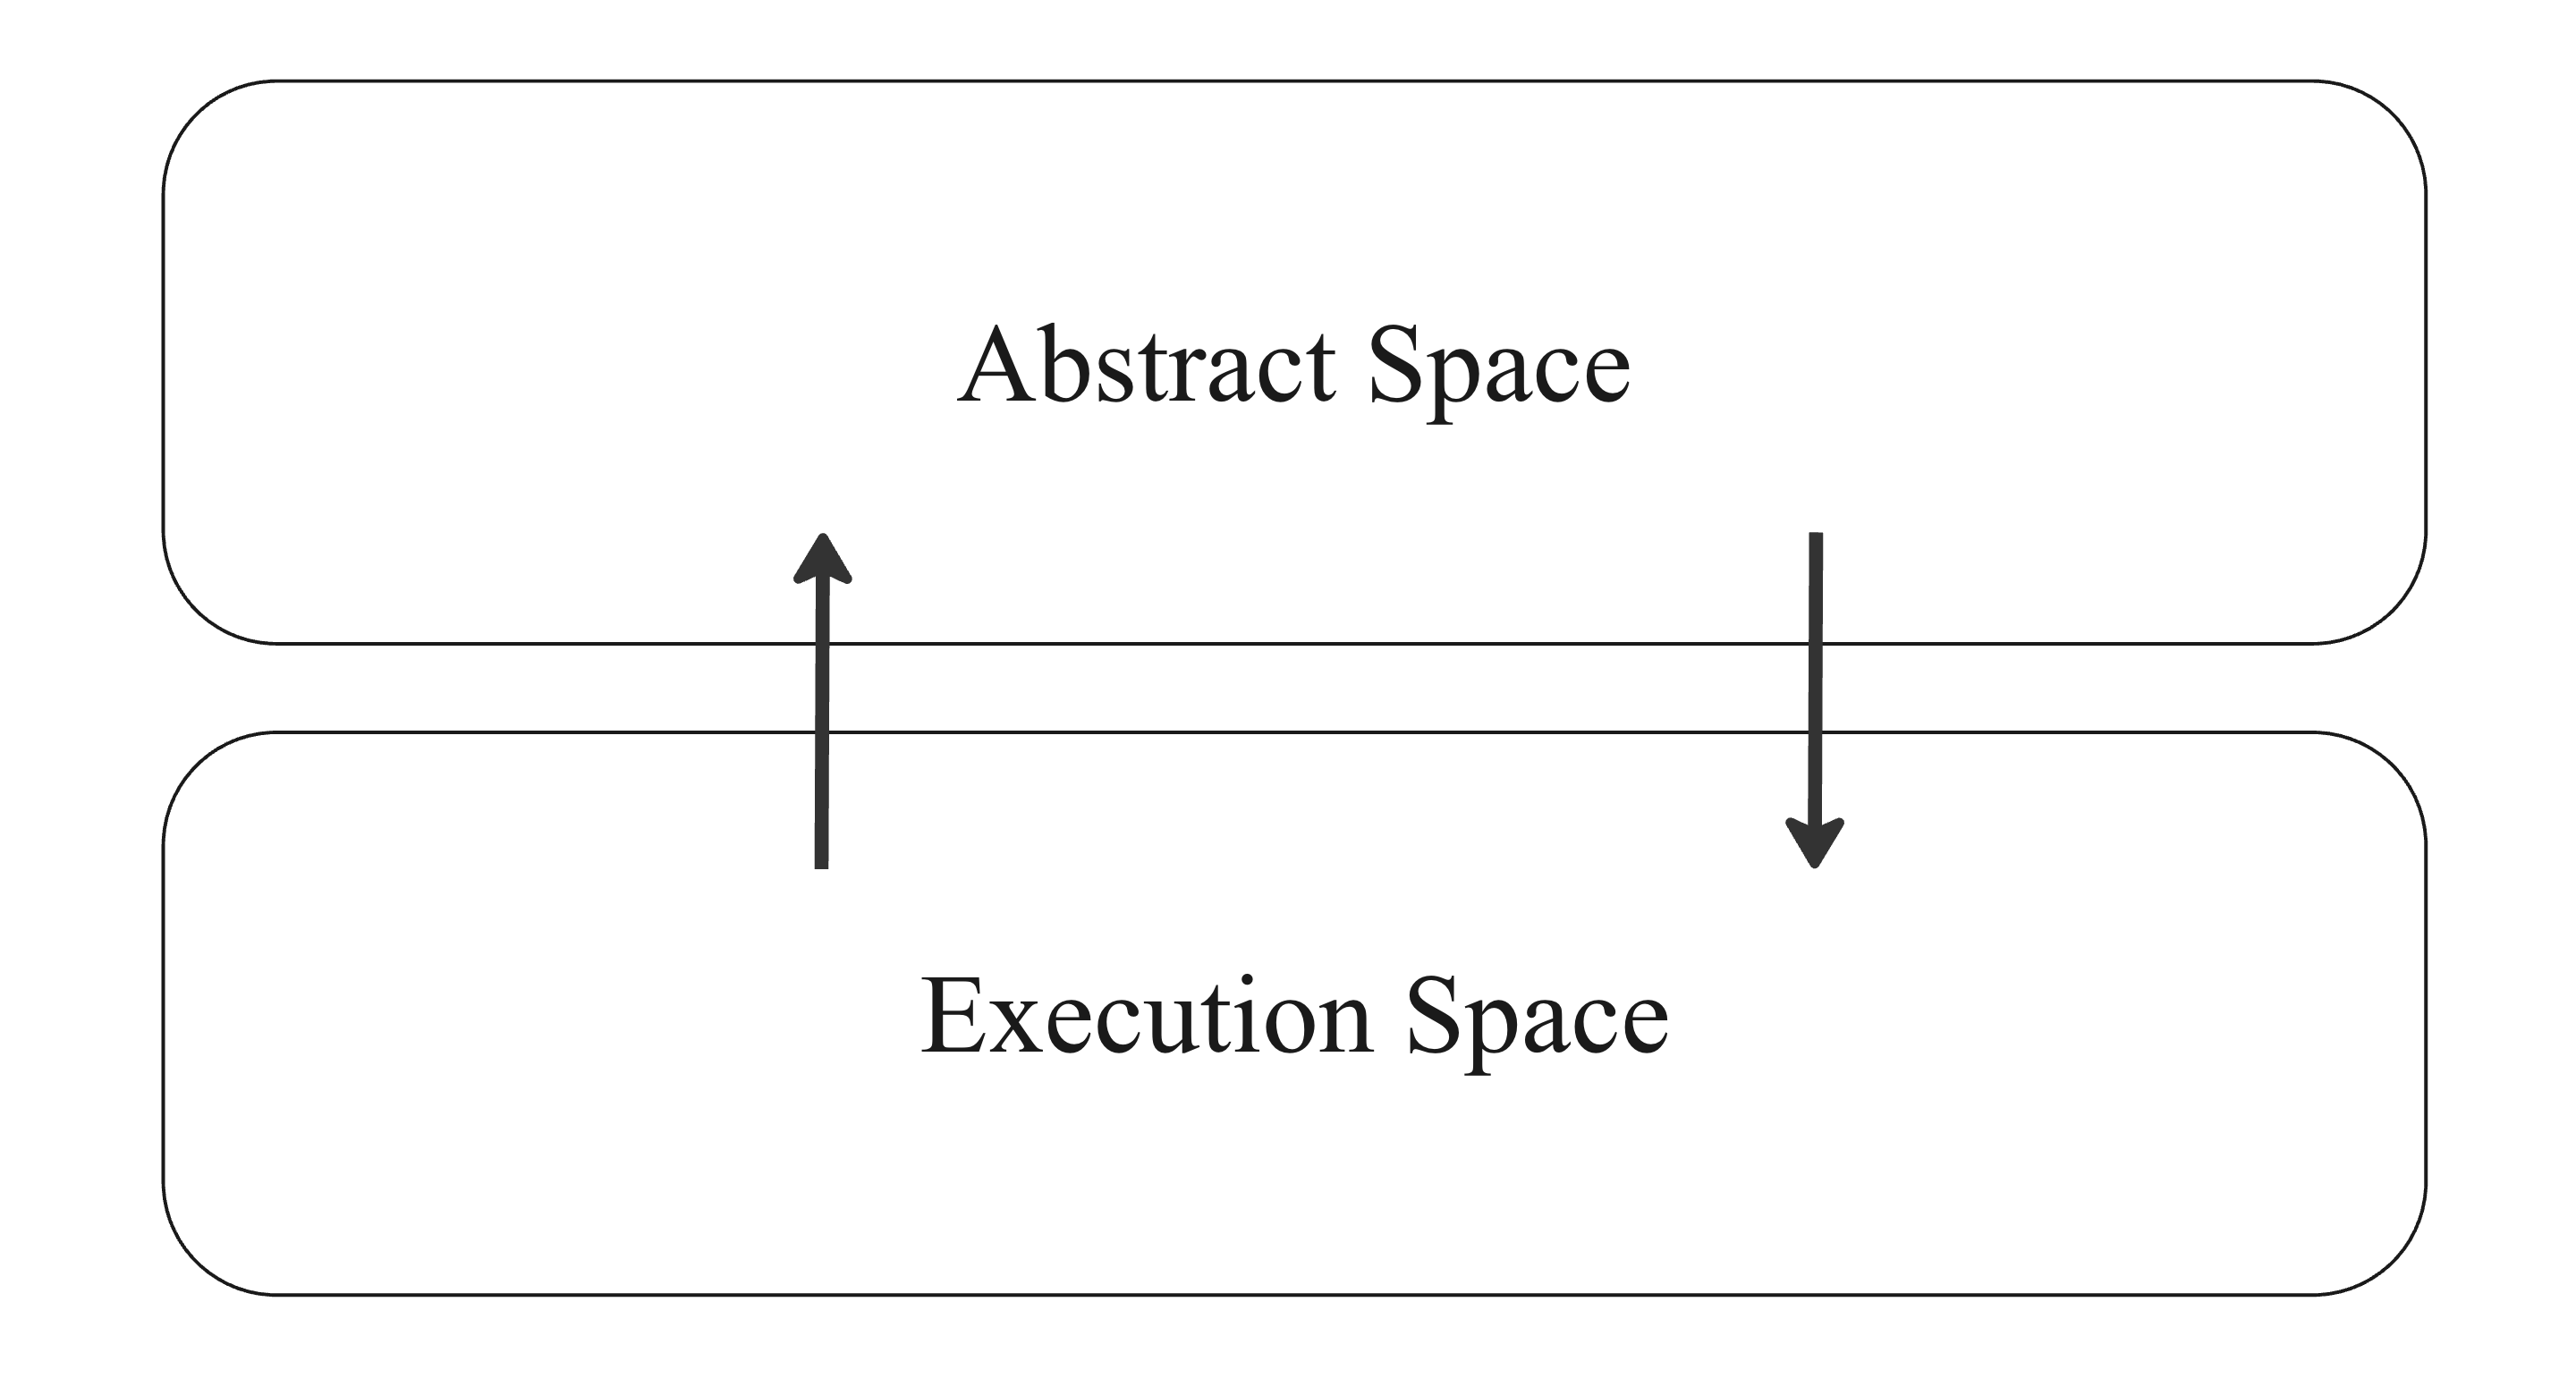
\includegraphics[width=1\linewidth]{twospaces.png}
\caption{Creative Processes Involve Moving Between Abstract Spaces and Execution Spaces}
\label{fig:enter-label}
\end{figure}

Creativity is largely a process of formulating ideas and intentions in the abstract space, then transitioning to the execution space to realise them. This process rarely follows a linear trajectory; instead, it typically involves iterative movement between these spaces. Actions in the execution space generate new concepts in the abstract space—including value judgments and novel ideas—which are subsequently explored further in the execution space, establishing a continuous, and often very tight, feedback loop between abstraction and execution.

This distinction offers a simple yet effective way to conceptualise human-AI co-creative roles. An observation from both this thesis and the broader literature is that, at least under current interaction paradigms, users tend to migrate toward higher levels of abstraction, like ideating and planning, while outsourcing tasks at the execution level to the AI, such as writing words, code or drawing pixels. Indeed, it is often said both by commentators and even AI companies that the value of AI "reducing the gap between idea and execution".

This arrangement presents certain advantages, enabling individuals to realise their creative ideas even when they lack specific technical skills or resources. For instance, a person may conceive compelling ideas for films or short stories but struggle with the writing process itself. However, this division of labour, where users adopt primarily directive and ideation roles in the abstract space, may potentially erode skills and self-efficacy, ultimately diminishing creative satisfaction.

An illustrative example was provided by a participant in one of the studies discussed in Chapter 4. When describing how Vorges, the co-creative AI, performed most of the writing while they provided the ideas, they stated: "[it] made me feel like I was cheating somehow. It does not feel like my work, even though I gave all the ideas. Also, I believe there is satisfaction in putting a lot of effort/dedication/patience into something. Vorges made everything so simple, fast, and easy that it felt artificial and no real satisfaction came as a result." Another participant claimed their role was "like giving the recipe of a cake to someone and letting it do it."


In an extensive survey of roles assumed by humans and generative AI, \cite{Palani2024-on} describe users describe themselves as "ideators and project managers with a larger creative vision orchestrating information context and tasks across multiple GenAI models instead of traditional workers executing each task". 

However, this means that users are generally becoming less involved at execution levels. An emerging trend in coding, for example, which Andrej Karpathy has termed "vibe coding", involves: 

\begin{quote}
"[I] forget that the code even exists. It's possible because the LLMs (e.g. Cursor Composer w Sonnet) are getting too good. Also I just talk to Composer with SuperWhisper so I barely even touch the keyboard. I ask for the dumbest things like "decrease the padding on the sidebar by half" because I'm too lazy to find it. I "Accept All" always, I don't read the diffs anymore. When I get error messages I just copy paste them in with no comment, usually that fixes it. The code grows beyond my usual comprehension, I'd have to really read through it for a while. Sometimes the LLMs can't fix a bug so I just work around it or ask for random changes until it goes away. It's not too bad for throwaway weekend projects, but still quite amusing. I'm building a project or webapp, but it's not really coding - I just see stuff, say stuff, run stuff, and copy paste stuff, and it mostly works."
\end{quote}

While this can be considered a natural progression of coding, moving to higher levels of abstraction, research suggest this reduced involvement and diminished cognitive effort can lead to more errors and loss of cognitive skills \cite{Lee2025-dwL} Instead, some practitioners propose a more productive and long term beneficial approach involved engaging iteratively with the model \cite{Osmani2024-br}. 

Indeed, while AI itself, as a cognitive automation technology may offer a path of least resistance towards less involvement at the execution space, interaction design can also significantly impact this. For example, the participants in my study who reported less involvement were using a control version of the co-creative system which only enabled interaction via chat, primarily leading the user to adopt tasks in the abstraction space: giving ideas, feedback, and value judgements. In contrast, a user employing a version of the tool enabling both collaborative editing and chat, who reported engaging deeply in writing at the execution space, observed: "It forced me to put in some effort and do the majority of the work, I enjoyed how I could not be fully reliant on AI to provide me with all the text." Another participant using the same version claimed: "I really-really enjoyed writing this. I even had a deep moment of reflection, my writing was nostalgic and sad, but I was able to use AI to steer it in the right direction, it gave me confidence that I was also writing with correct grammar and spelling, English is not my first language and while I am proficient, I can still use proofreading to ensure good quality." Both of these participants, reported they did most of the work but AI helped them with suggestions, editing and other supportive tasks. 

These contrasting experiences highlight what I propose may be \textbf{fundamental tension of human-AI co-creativity}:

\begin{quote}
    As AI can increasingly assume complex roles within the creative process; users tend to move up levels of abstraction and adopt more directive roles, while they outsource execution-level roles to the AI. On one hand, this can help augment human creativity by helping them realise their ideas faster and with less resources. On the other hand, it may hinder their creativity by increasing errors, reducing quality, and eroding critical creative skills, agency, and satisfaction.
\end{quote}

When designing co-creative systems, designers, developers, and researchers must consider this \textbf{fundamental tension in human-AI co-creativity}. A critical observation in my research and in the literature is that facilitating user engagement at both the abstract spaces and execution spaces may be an effective strategy to address this fundamental tension, helping them realise the beneficial co-creative potential of AI while reducing the shortcomings of increased creative and cognitive offloading. A promising alternative is enabling both collaborative spaces and communication spaces, where interaction through and about the creation are separated. However, how to effectively implement this in practice remains an important area for further research. 

\subsubsection{Stages}

A second conceptual dimension of the framework recognises that creative processes progress through different stages, with AI potentially assuming distinct tasks at each stage. Various stage-based models of creativity have been proposed in the literature, but for simplicity, this framework distinguishes between divergent and convergent stages.

A few examples from throughout this thesis offer an illustration of what factors may lead to the human and the AI to assume certain roles within each stage. For example, the designers working with Tilly in the case study described in Chapter 6 system initially utilised it to ideate novel designs for complex briefs both conceptually and visually—a divergent process—and found this application highly valuable. However, they encountered greater challenges during convergent processes, when they wanted to produce final renders, and editable files. Largely this was the result of limitations in the interface and the underlying generative model that failed at effective non-destructive iteration of outputs. It was also not fundamentaly able to produce 3D vector models which are considered the final stage of their process (before manufactoring). 

In creative writing participants in the "Beyond chat" study described in Chapter 4, employed AI primarily to polish drafts \textit{they had initiated}, thus engaging AI during a \textit{convergent} stage, mainly when they interacted with it throug both a chat and a collaborative text editor. In contrast, users of chat-only interfaces reported using AI as a brainstorming partner—a divergent application. 

Lastly, in the installation case studies described earlier, AI was utilised predominantly in convergent stages to execute performances, while the ideation stage remained primarily human-driven. This case, being a new type of creative practice, warrants further discussion that will be treated in later section.

\subsubsection{Spaces and Stages Integration}

Integrating these two dimensions produces a model with abstract and execution spaces on the vertical axis and divergent and convergent stages on the horizontal axis. AI roles can be roughly positioned within this grid, with the understanding that roles may shift over time, and AI can move between positions throughout a single interaction. In some cases, this movement occurs fluidly, while in others, the affordances of the tool may constrain the AI to a more fixed position.

\begin{figure}
    \centering
    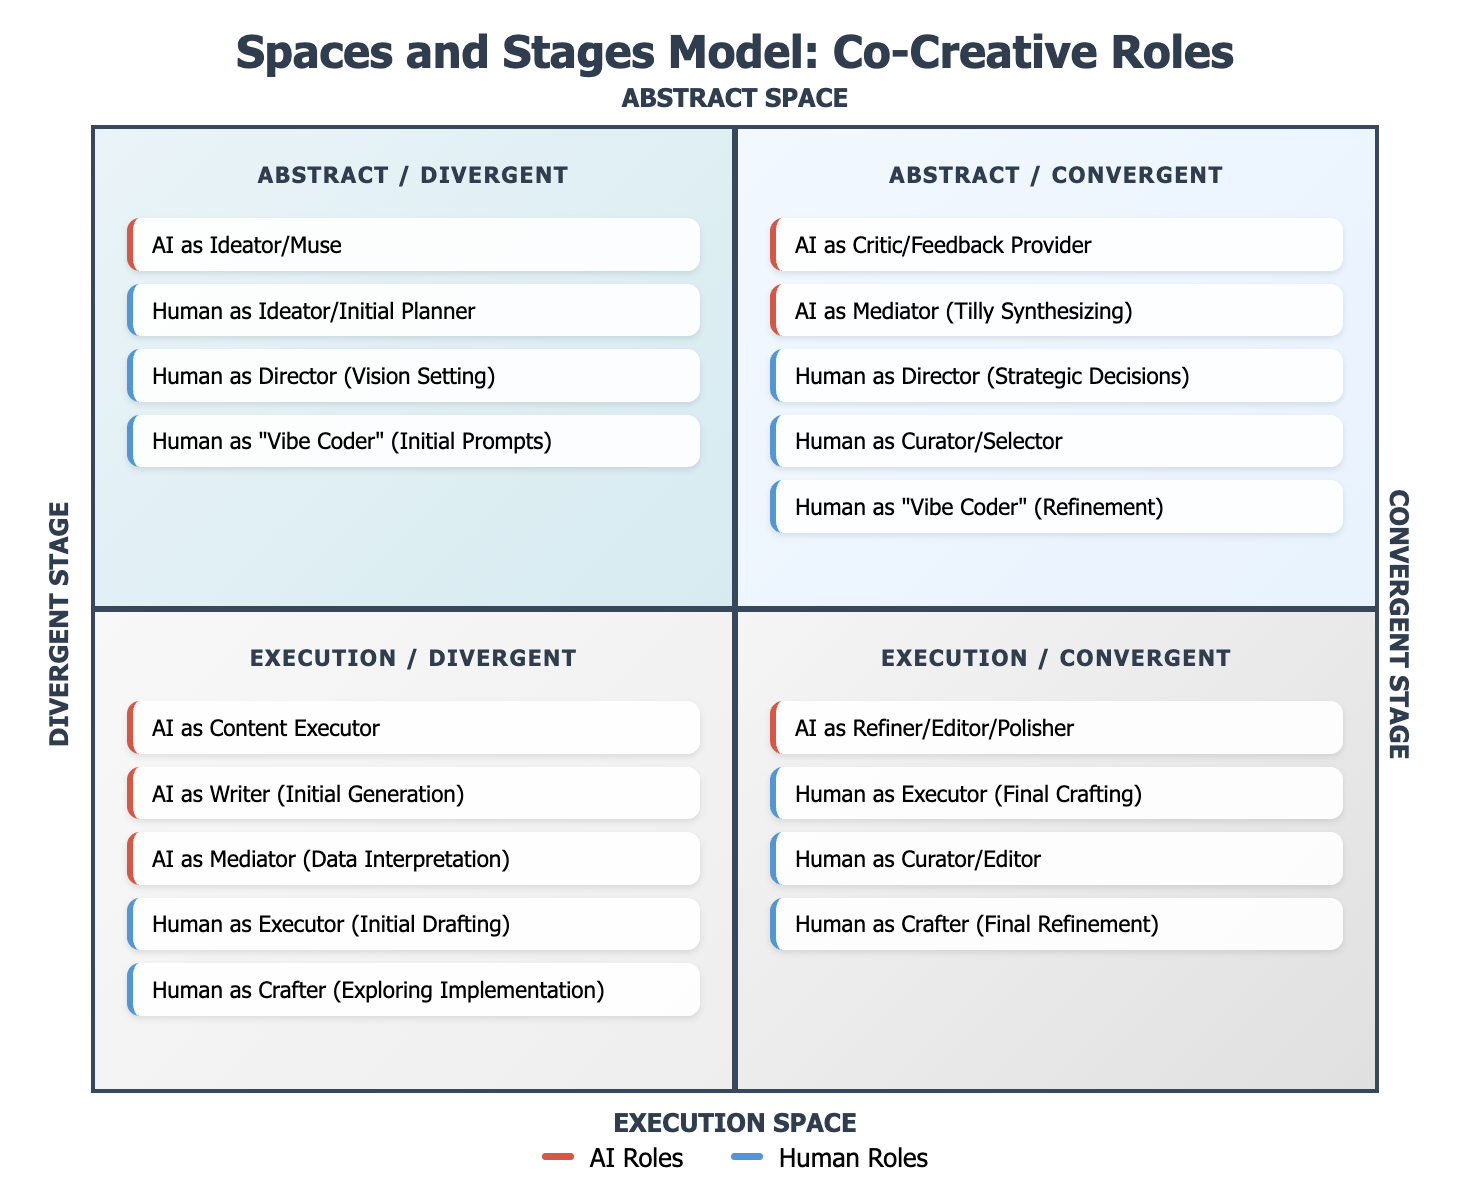
\includegraphics[width=1\linewidth]{spacesandstages.png}
    \caption{Spaces and Stages Model, showing different roles in each quadrant}
    \label{fig:enter-label}
\end{figure}

The notion of spaces is well-established in creativity research and computational creativity literature, particularly in Boden's conceptual spaces theory, which was later formalised by Wiggins. While this thesis does not offer an exhaustive mathematical formalisation of abstract and execution spaces (such as Wiggins's conceptual spaces mathematical formalisation), it is worth noting that both can be understood within the broader framework of conceptual spaces proposed by both him and Boden.

In Wiggins' formalisation, conceptual spaces encompass both unrealised and realised artifacts, with a set of rules governing exploration and transformation between these states. Drawing a preliminary parallel, the abstract spaces proposed in this model can be understood as including both unrealised and realised artifacts at a conceptual level, while execution spaces may comprise the rules and mechanisms of exploration that facilitate the transition from unrealised to realised artifacts.

This distinction is important to the core argument made here: that both working at the abstract and execution level is important. It is useful for a creative to know the rules (execution space) for how to traverse the conceptual space they are working in and not merely act in the abstract space. For example, it is useful for a musician to know music theory, how to use scales, and how to play an instrument. While an AI may abstract this away, enabling a user to merely say: "play an upbeat song", this will likely constrain their potential to meaningfully explore, and transform the space. This does not mean that knowing these rules is a prerequisite. In fact, not knowing the rules may be conducive to breaking them. However, within the observations in my research and in the emergent literature, AI automating the application of these rules, and prioritising interactions only at the abstract space presents the risk of increasingly separating the users from the execution space, becoming alienated from the artefact itself, and assuming only directive or instructing roles. 


\subsubsection{Narrow vs. General AI Co-Creators}

This framework is useful for another categorisation of roles which I offer here. Within each quadrant of the spaces-stages framework, different tasks can be located. A role corresponds to assuming one or more tasks within a particular region. Many previous role classifications were developed in a technological landscape where computational algorithms were constrained to specific, narrow tasks. However, newer generations of algorithms give rise to co-creators capable of moving across tasks and stages of the creative process, rather than merely automating isolated components.

For example, whereas earlier systems might focus exclusively on generating ideas, or merely generating an image, new emerging more capable systems can assist users across both abstract and execution spaces and across divergent and convergent stages level. I propose we are witnessing a gradual transition from narrow to general AI co-creators.
While increasingly, there is potential for AI systems to engage in a general level, moving across spaces and stages, this hinges on their capacity to engage in full-dialogic co-creativity [explain this further].

With this: I propose the following: 

\begin{quote}
    \textbf{A narrow AI co-creator} is a type of role that primarily occupies a fixed position within the Spaces and Stages Model, assuming specific and narrowly defined tasks, and which generally is not robust across the six dimensions of co-creativity
\end{quote}

\begin{quote}
    \textbf{A general AI co-creator} is a type of role that is high across the six dimensions of co-creativity, and which can engage with the user at the abstract and execution spaces, and across divergent and convergent stages. 
\end{quote}


\section{Final thoughts}

This thesis provided a mixed methods research approach to address the fundamental question of effective human-AI co-creativity. I focused on the domains of writing, visual production and new media installations. Each provided different insights, from both a practice-based research perspective and from a design research perspective. 

These insigts were collated into a set of 12 design principles for co-creative AI, aiming to fill the gap in such principls that exist for other domains of HCI but not in human-AI co-creativity. 

These principles are not meant to be fixed or all-ecompassing. They merely address the most pressing issues prevalent now, and the ones I was able to observe throughout my research. Undoubtedly, as capabilities advances and increasingly more research is focused on this area, the principles might change, or expand, or become trivial. 

However, they provide a foundational underpinning that frames our relationship with generative tools as a dialogic one, where human creativity is prioritised, enhanced and highly valued. 



